\documentclass[12 pt]{article}
\usepackage[left=2.66cm,top=3cm,right=2.66cm,bottom=3cm,bindingoffset=0.5cm]{geometry}

\usepackage{graphicx}
\usepackage{setspace}
\usepackage{hyperref}
\usepackage{enumitem}
\onehalfspacing

\begin{document}
	
	\begin{center}
		
		\begin{Huge}
		\textbf{HCCO}
		\end{Huge}
			
		\begin{Large}
		\textsc{IN INTERSTELLAR SPACE\linebreak}
		\end{Large}
		
		\begin{scriptsize}
		$
		\textsc{Divya Raj }\bullet\textsc{ David Nallapu }\bullet\textsc{ Simran Srivastava }\bullet\textsc{ Anushree Avasthi }\bullet						\textsc{ Bhavya Aggarwal}	
		$
		\end{scriptsize}
				
	\end{center}
	
	\section*{Structure}
		The  ketenyl  radical(HCCO) has  a  planar  structure  with  a  practically  linear  CCO  backbone  and  the  H  atom  lying  out  of  			the	linear  axis.  The  radical  has a ${}^2A''$ ground  electronic  state  and a  complex  rotational  structure  whose $N_{K_a,K_c}$ 			levels  split in  a	fine (electronic spin-rotation interaction) and hyperfine (H nuclear  spin)  structure  described  by  the  quantum  		numbers J and F, respectively.
		
		\begin{figure}[h!]
		  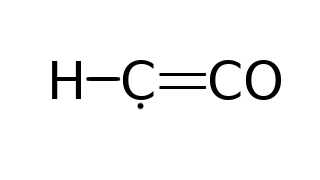
\includegraphics[width=50mm]{hcco.png}
  			\centering
  			\caption{The Ketenyl readical, Lewis structure }
  			\label{fig:PublicKey-Basic}
		\end{figure}
		
	\section*{Interstellar Sources of Detection}
		HCCO was first detected in the starless core Lupus-1A and the molecular cloud L483.\cite{mcg}
		
	\section*{Observation Techniques}
		The observation which led to the discovery of the molecule in interstellar space were ground based and were carried out using the
		\href{https://en.wikipedia.org/wiki/IRAM_30m_telescope}{IRAM 30m}
		millimeter radio telescope, located in Veleta, Granada Province, Spain.\cite{IRAMwiki}
		\\The observations were made in selected frequency ranges from 83 to 105 GHz, which fall under the Ultra high frequency 
		range.\cite{EMwiki}
		
	\begin{thebibliography}{999}
	\bibitem{mcg}
 	 Marcelino Agúndez, José Cernicharo, and Michel Guélin, \emph{Discovery of interstellar ketenyl (HCCO), a surprisingly abundant radical}.
 	 April, 2015.
	
	\bibitem{IRAMwiki}
	Wikipedia - \href{https://en.wikipedia.org/wiki/IRAM_30m_telescope}{IRAM 30m telescope}
	
	\bibitem{EMwiki}
	Wikipedia - \href{https://en.wikipedia.org/wiki/Electromagnetic_spectrum}{Electromagnetic Spectrum}	
	\end{thebibliography}
	
\end{document}
